% Motivation figure: source images are embedded unchanged from slide 3 of
% deck/dissertationv3.pptx. The portrait is selected with a LaTeX viewport;
% the prompt excerpt is editable vector text rather than raster lettering.
% Rebuild from repository root with pdflatex and output-directory=build/figures.
\documentclass[border=0pt]{standalone}
\usepackage[T1]{fontenc}
\usepackage{newtxtext,newtxmath}
\usepackage{graphicx,xcolor}
\definecolor{otblue}{HTML}{0072B2}
\definecolor{otgray}{HTML}{5A5A5A}
\newcommand{\paneltitle}[1]{{\fontsize{12}{14}\selectfont\bfseries #1}}
\newcommand{\panelnote}[1]{{\fontsize{10.5}{12}\selectfont\color{otgray}#1}}
\setlength{\parindent}{0pt}
\setlength{\fboxsep}{7pt}
\begin{document}
\begin{minipage}{16.3cm}
\begin{minipage}[t][5.25cm][t]{7.95cm}
  \paneltitle{(a) Verbal description}\par\vspace{0.16cm}
  \begin{minipage}[c][4.05cm][c]{3.05cm}
    \centering
    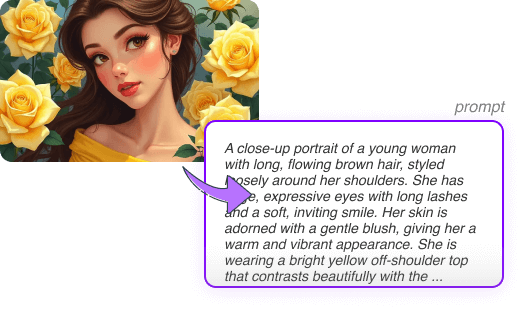
\includegraphics[width=3.05cm,viewport=0 148 200 311,clip]{figures/introduction/long_prompt_slide.png}\par
    \vspace{0.14cm}
    \panelnote{A visual idea}
  \end{minipage}%
  \begin{minipage}[c]{0.48cm}
    \centering\color{otblue}\fontsize{12}{14}\selectfont$\rightarrow$
  \end{minipage}%
  \colorbox{otblue!5}{%
    \begin{minipage}[c][3.62cm][c]{3.90cm}
      {\fontsize{10.5}{12}\selectfont\bfseries\color{otblue}Prompt excerpt}\par\vspace{0.08cm}
      {\fontsize{11}{13}\selectfont\raggedright
      ``A close-up portrait of a young woman with long, flowing brown hair, styled loosely around her shoulders.\ \ldots\ She is wearing a bright yellow off-shoulder top\ \ldots''\par}
    \end{minipage}%
  }\par\vfill
  \panelnote{Expressing visual detail can require many words.}
\end{minipage}%
\hspace{0.4cm}%
\begin{minipage}[t][5.25cm][t]{7.95cm}
  \paneltitle{(b) Beyond verbal description}\par\vspace{0.16cm}
  \begin{minipage}[c][4.05cm][c]{7.95cm}
    \centering
    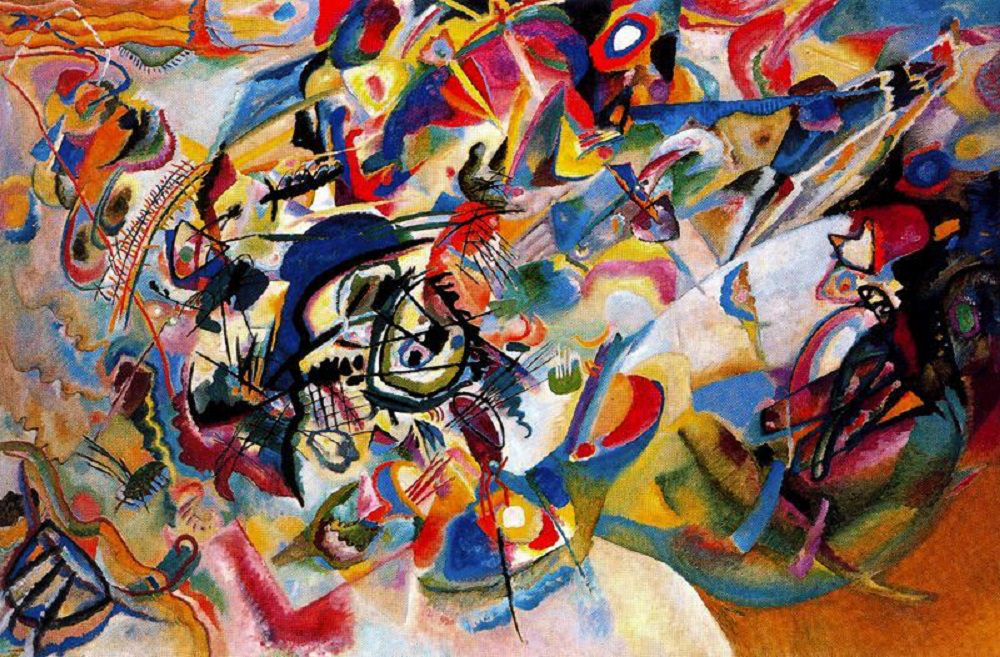
\includegraphics[height=3.67cm]{figures/introduction/composition_vii.png}\par
    \vspace{0.10cm}
    {\fontsize{10}{11.5}\selectfont\color{otgray}Wassily Kandinsky, \textit{Composition VII} (1913)}
  \end{minipage}\par\vfill
  \panelnote{Some visual qualities resist precise verbal description.}
\end{minipage}
\end{minipage}
\end{document}
